\documentclass[a4paper,11pt,dvipdfmx]{ujarticle}
% パッケージ
\usepackage{graphicx}
\usepackage{url}
% レイアウト指定を記述したファイルの読み込み
\input{layout}

% タイトルと氏名を変更せよ．
\title{日本におけるデジタル化の状況}
\author{G684602026 澤田　将希}

\begin{document}

\maketitle %ここにタイトルが入る

% ここから本文
\section{デジタル競争ランキング}\label{sec:imd}
% を使う

国際経営開発研究所(IMD)の調査\cite{imd}によると、日本のデジタル競争ランキングは図\ref{図1}に示すように、調査対象の64各国中、総合で28位、準備分野で27位となっている。

%  参考文献の参照: \cite{}
%  図番号の参照： \ref{}
% を使う
% 文献データベースのキーワードは oecd と imd
% になっている．
\cite{oecd,imd}
% 図の挿入
% \includegraphics{}
\begin{figure}[htbp]
\centering
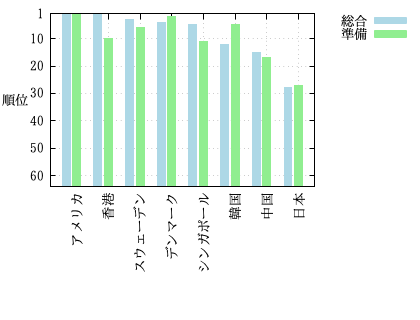
\includegraphics{fig51.png}
\caption{デジタル競争力ランキング}
\label{図1}   
\end{figure}
% を
% \begin{figure}[htbp]
% \end{figure}
% で囲み
% \caption{}
% で図のタイトルを入れる．
% \label{}
% を使って図番号が参照できるようにする
% また，
% \centering
% で図が中央に来るようにする

% ーーー
% 節見出し(2)
\section{ブロードバンドの整備状況}\label{sec:oecd}
% 本文(2)
OECDによるとブロードバンド回線の普及に関する調査\cite{oecd}によると、表\ref{表1}に示すように、日本における100人あたりのモバイルブロードバンドの加入者数は190.5で、第1位になっている。2位はエストニアで、3位米国と続く。
% 表の挿入
% \begin{tabular}
\begin{table}[htbp]
\centering
\caption{モバイルブロードバンドの加入者数(100人あたり)}
\label{表1}
\begin{tabular}{|c|c|c|}
    \hline
   実験  & 国名 & 加入者数 \\
    \hline
    1位 & 日本 & 190.5 \\
    2位 & エストニア & 179.9 \\
    3位 & 米国 & 169.0 \\
    4位 & フィンランド & 157.0 \\
    5位 & デンマーク & 141.7 \\
    6位 & ラトビア & 141.6 \\
    7位 & イスラエル & 139.9 \\
    8位 & オランダ & 133.7 \\
    9位 & ポーランド & 131.3 \\
    10位 & スウェーデン & 127.2 \\
    \hline
\end{tabular}
\end{table}
% \end{tabular}    
% による表の記述を 
% \begin{table}[htbp]
% \end{table}
% で囲み
% \caption{}
% で表のタイトルを入れる．
% \label{}
% を使って表番号が参照できるようにする
% また，
% \centering
% で表が中央に来るようにする
\section{考察}
\begin{itemize}
    \item \ref{sec:imd}からアメリカや香港などの他の国々と比較して、日本は国や企業のデジタル化する能力や準備が遅れていることから、日本のデジタル化があまり進んでないと考えられる。
    \item \ref{sec:oecd}から他国と比較して、日本はモバイルブロードバンドの加入者数が多く、高速通信の環境が他国より整っていると考えられる。
    
\end{itemize}
% ーーー
% 見出し(3)
% 考察
%
% \begin{itemize}
% \end{itemize}
% を使って箇条書きで記述する

% ここに参考文献が入る
%
\bibliographystyle{junsrt}
\bibliography{exercise.bib}

\end{document}